\chapter{A gestão das operações em ambiente industrial - primeiros conceitos}
\label{chap:gestao_operacoes}

O pacote de valor é definido como sendo um conjunto de bens e serviços fornecidos, em variadas proporções, para os clientes. Desta forma as empresas que prestam serviços ou fornecem produtos passam a fornecer outros itens que agregam e consolidam as relações com seus clientes.
Apesar do pacote de valor fortalecer essas relações é necessário que as empresas expandam os mesmos fornecendo mais benefícios aos clientes.

\begin{figure}[H]
    \caption{Fluxo da geração do pacote de valor.}
    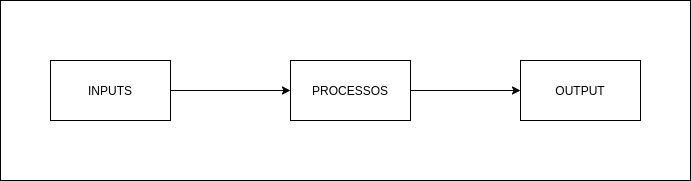
\includegraphics[width=\textwidth]{images/pacote_valor.png}
    \label{fig:pacotevalor}
    \legend{Fonte: Adaptado de \cite{slack2006administracao}.}

\end{figure}

O modelo de \textit{input}-processo-\textit{output} da Figura \ref{fig:pacotevalor} auxilia a compreensão da atividade da produção. Os \textit{inputs} representam recursos do processo produtivo, divididos em recursos de transformação (informações, matéria prima, componentes e clientes) e recursos transformadores (equipamentos, máquinas, construções e equipe de trabalhadores). O Processo envolve todo o procedimento de transformação dos recursos, planejamento, projeto e controle, e é a parte que é executada dentro da empresa. O \textit{Output} é a saída, o pacote de valor (bens ou serviços) destinado ao cliente ou distribuidora. \cite{slack2006administracao}.

%------------------------------------------------------------------
\section{Aplicação Prática}
\label{sec:gestao_operacoes_aplicacao}
O pacote de valor da empresa SunBurn revolve entorno da produção e venda de energia elétrica bem como serviços agregados. No território nacional, esta empresa produz energia elétrica através da produção solar e eólica, a qual é fornecida para a empresa distribuidora regionalmente instalada.

Acredita-se que o pacote de valor da empresa pode ser expandido através da integração das tecnologias de produção de forma que ela possa garantir o fornecimento da energia que vende mesmo quando algum incidente ocorra na geração através de uma das tecnologias. O atual uso de diferentes fontes limpas de energia poder ser realizado de forma integrada criando uma redundância do sistema de produção da Sunburn. Esta integração pode então ser vendida como um serviço adicional de aumento na garantia da entrega de energia para o cliente.

Por outro lado, a SunBurn já possui um estudo para a formação de micro-geradoras de energia elétrica, as quais são implantadas direto no cliente final. Tal modo de produção viabiliza a redução dos custos agregados na transmissão e distribuição de energia elétrica para o cliente, além de possibilitar uma redundância local no fornecimento de energia para o cliente em questão. Esse modo de geração de energia, poderá ser amplamente utilizado pela SunBurn após a regulamentação local da venda de energia elétrica produzida por essas micro-geradoras para as empresas de transmissão e distribuição. A SunBurn poderá oferecer os seus serviços de regulação, controle e manejo do fornecimento de energia para os seus clientes que possuam usinas micro-geradoras, de forma que os clientes possam vender o excedente de energia gerado em seus territórios.

\begin{figure}[H]
    \caption{Diagrama do \textit{input}-processo-\textit{output}}
    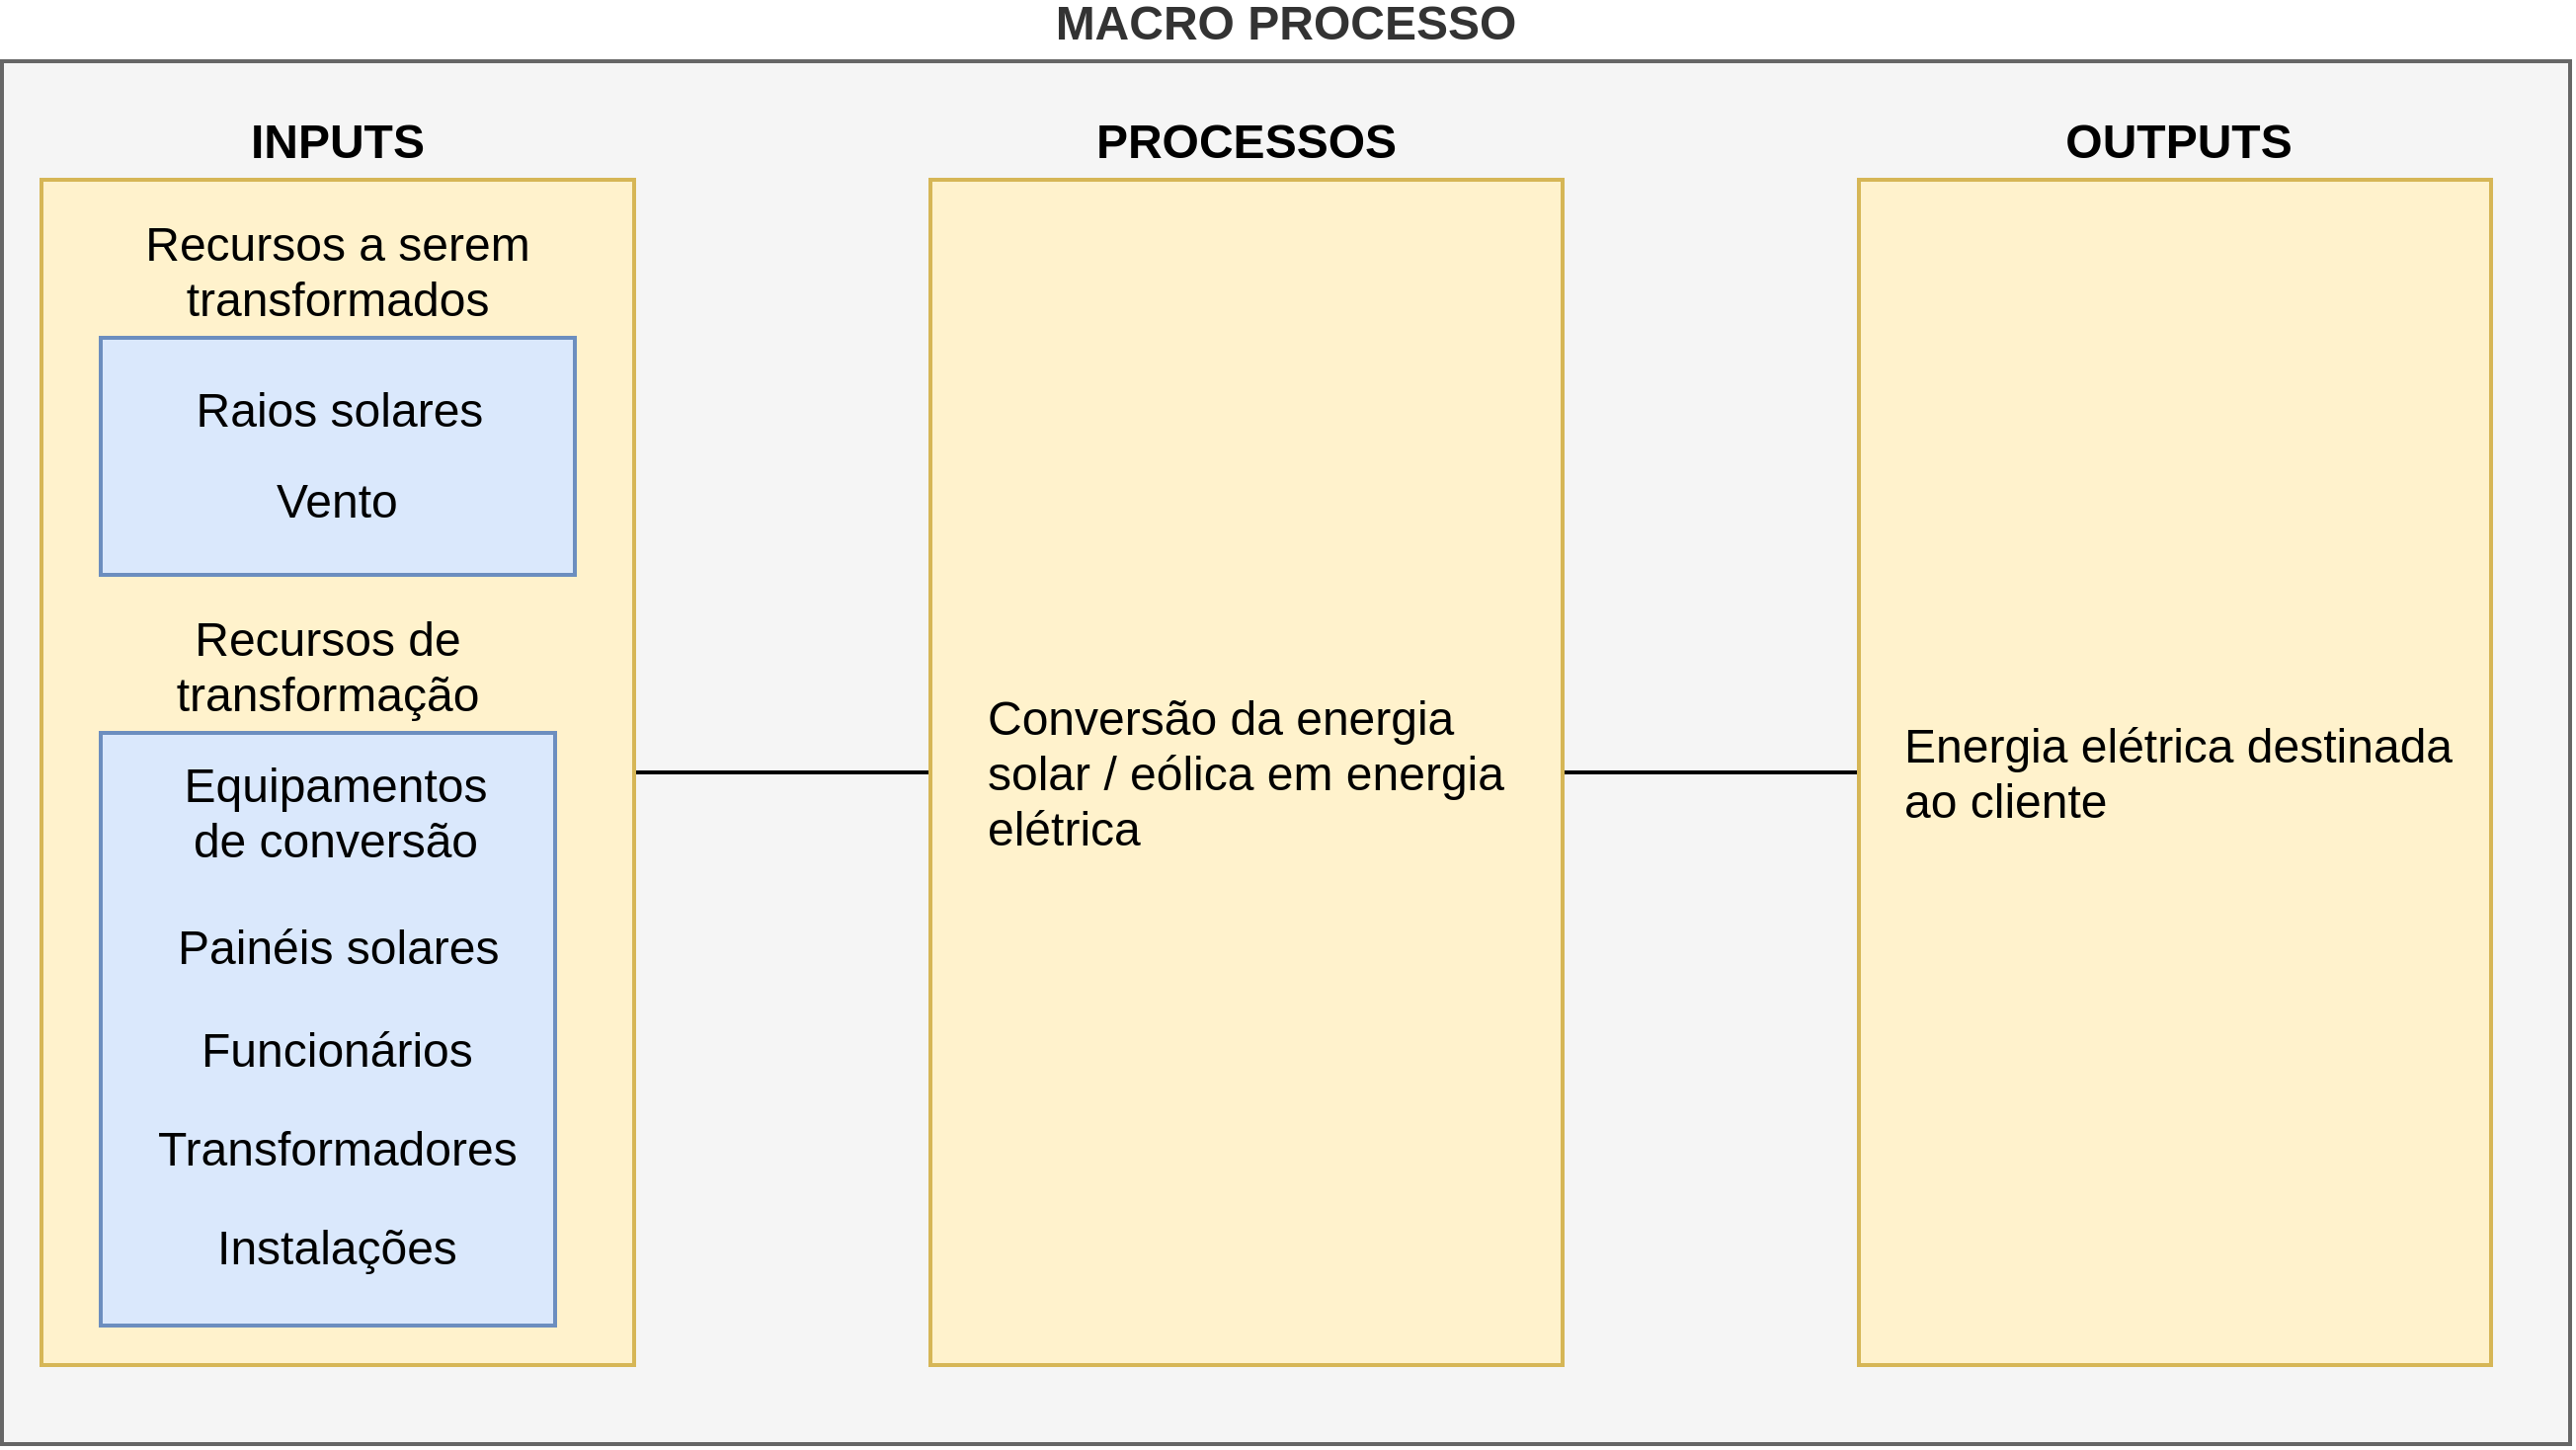
\includegraphics[width = 1\textwidth]{images/diagram.png}
    \legend{Fonte: Autoria própria.}
    \label{fig:gestao_operacoes_aplicacao_diagrama}
\end{figure}

O macro processo da empresa pode ser observado na Figura \ref{fig:gestao_operacoes_aplicacao_diagrama}. Os recursos de energia renovável somados aos recursos transformadores compõem os \textit{inputs} que serão usados e transformados pela etapa de processos. Possuindo estes recursos, a empresa realiza o processo de conversão da energia atual em elétrica, para assim gerar a saída (\textit{output}) que é destinada ao cliente.


% \subsection{Requisitos do cliente}
% \label{sub:reqc}
